\documentclass[11pt]{article}
\usepackage[final]{acl}
\usepackage{times}
\usepackage{latexsym}
\usepackage[T1]{fontenc}
\usepackage[utf8]{inputenc}
\usepackage{microtype}
\usepackage{inconsolata}
\usepackage{graphicx}
\usepackage{booktabs}
\usepackage{multirow}
\usepackage{amsmath}
\usepackage{url}


\title{RUN: An Unsupervised Pipeline for Roman Urdu Normalization\\
with Code-Switching Awareness}

\author{
  Basima Maham \\
  CS Department, Lahore \\
  \texttt{basimamaham@gmail.com} \\\And
  Tahreem Fatima \\
  CS Department, Lahore \\
  \texttt{tahreem29fatima@gmail.com} \\\AND
  Soban Khan \\
  CS Department, Lahore \\
  \texttt{thunderstorm20115@gmail.com} \\
}

\date{}

\begin{document}
\maketitle

% ────────────────────────────────────────────────────────────────
\begin{abstract}
Roman Urdu --- Urdu written in Latin script --- is the dominant mode of informal communication on Pakistani social media, yet it poses significant challenges for natural language processing due to extreme orthographic inconsistency and pervasive code-switching with English. A single word may appear in dozens of spelling variants across users and platforms, making downstream tasks such as sentiment analysis, machine translation, and information retrieval unreliable without a normalization step. We present RUN (Roman Urdu Normalizer), an unsupervised preprocessing pipeline that learns normalization rules directly from unannotated social media text without requiring any labeled training data. RUN 
combines character-level FastText embeddings, centroid-based clustering, and a hybrid canonicalization strategy incorporating phonetic similarity and edit distance to construct a dictionary of 7,354 normalization rules from a corpus of 220,667 sentences. A sentence-level language detection mechanism allows RUN to preserve English tokens intact, making it robust to the code-switched nature of Pakistani online text. Evaluated on 200 human-annotated sentences, RUN achieves an F1 score of 83.9\%, outperforming rule-based, edit-distance, and large language model baselines, including Claude, Gemini, and DeepSeek. RUN covers 97.1\% of tokens in our test set, compared to 72.2\% for the strongest rule-based baseline.
\end{abstract}

% ────────────────────────────────────────────────────────────────
\section{Introduction}
The rapid growth of social media in Pakistan has produced an enormous volume of user-generated text written in Roman Urdu — a non-standardized romanization of Urdu that has no official orthography, no agreed-upon spelling conventions, and no fixed vocabulary boundaries. Users write the same word however, it sounds to them: bohat, buhut, bhot, and bht are all attested spellings of the Urdu word for "very," and all appear frequently in the same corpus. This orthographic freedom, while natural for human communication, makes Roman Urdu one of the most challenging low-resource language varieties for automatic processing.

The challenge is compounded by code-switching. Pakistani social media users routinely mix Roman Urdu and English within a single sentence, sometimes within a single clause. A sentence like "yaar mujhe seriously tension ho rhi hai exams ki" contains English lexical items (seriously, tension, exams) embedded in an otherwise Urdu grammatical frame. Any normalization system that does not account for this mixing risks corrupting English tokens — replacing "to" with "toh" or "or" with "aur" in sentences where those words are functioning as English, not Urdu.

Despite the scale of Roman Urdu text production — hundreds of millions of speakers across Pakistan and the Pakistani diaspora — the language variety remains severely under-resourced. Labeled datasets are scarce, annotation is expensive and requires specialized expertise, and the informal register of social media text makes direct application of formal Urdu NLP tools ineffective. These constraints make supervised approaches impractical at scale and motivate the development of unsupervised methods that can learn from raw text alone.

Normalization is a critical preprocessing step for virtually every downstream NLP task. Sentiment classifiers trained on clean text fail when confronted with "bht accha tha" if they have never seen bht as a variant of bohat. Machine translation systems produce degraded output when the source is riddled with inconsistent spellings. Search and retrieval systems miss relevant documents because query terms and document terms do not match. A reliable normalization layer that maps the long tail of spelling variants to a canonical form would benefit the entire Roman Urdu NLP ecosystem.

We present \textbf{RUN} (Roman Urdu Normalizer), an unsupervised pipeline that addresses this problem without requiring any annotated data. RUN learns a dictionary of normalization rules from a raw corpus of 220,667 sentences by combining character-level FastText embeddings, centroid-based clustering, and a hybrid canonicalization strategy. A sentence-level language detection module identifies English-dominant contexts and freezes English tokens, handling code-switching explicitly rather than treating the input as monolingual.
The contributions of this paper are as follows:
\begin{itemize}
\setlength{\itemsep}{0pt}
\setlength{\parsep}{0pt}
\setlength{\parskip}{0pt}
    \item We present the first fully unsupervised Roman Urdu normalization pipeline with explicit code-switching awareness, requiring no labeled training data.
    \item We construct a normalization dictionary of 7,354 rules learned entirely from unannotated social media text through four rounds of iterative error-guided refinement.
    \item We conduct a systematic comparison against five baselines — manual rules, edit distance, and three large language models (Claude, Gemini, DeepSeek) — on a held-out test set of 200 human-annotated sentences, where RUN achieves the highest F1 score of 83.9\%.
    \item We provide an honest discussion of evaluation limitations, including the recall metric bias introduced by using RUN's own output as the normalization reference.
\end{itemize}


% ────────────────────────────────────────────────────────────────
\section{Related Work}
Roman Urdu normalization sits at the intersection of three research areas: text normalization for noisy user-generated content, code-switching in South Asian languages, and low-resource NLP for romanized scripts.

\textbf{Text Normalization for Social Media.} Normalization of non-standard text has been studied extensively for English social media. \citet{han2011lexical} introduced a lexical normalization system for English tweets using string similarity and context, establishing the core precision-recall tradeoff that remains central to evaluation in this space. \citet{sproat2017rnn} demonstrated that while RNN-based normalizers achieve high overall accuracy on speech text normalization, they remain prone to catastrophic errors on unseen patterns — a finding that motivates the interpretable, dictionary-based approach we take in RUN. These methods generally assume a well-defined standard variety as the normalization target and rely on labeled parallel corpora — assumptions that do not hold for Roman Urdu, where no official standard exists and labeled data is absent.

\textbf{Roman Urdu Processing.} Roman Urdu presents unique challenges because it has no official orthographic standard. The most directly related prior work is \citet{khan2019clustering}, who present a clustering framework for lexical normalization of Roman Urdu using UrduPhone — a phonetic encoding scheme for Roman Urdu — combined with their Lex-Var clustering algorithm. Their framework achieves F-measure gains of up to 15\% over baseline methods on four real-world datasets. RUN builds directly on their UrduPhone component for canonical form selection and is inspired by their clustering approach, though we replace Lex-Var with FastText embedding-based centroid clustering, which does not require predefined phonetic features. \citet{sharf2018lexical} provide further evidence of the scale of orthographic inconsistency in Roman Urdu and the difficulty of constructing normalization rules manually. \citet{shahroz2020rutut} developed RUTUT, a rule-based Roman Urdu to Urdu translator, demonstrating that rule-based systems can achieve reasonable coverage but require extensive manual construction and do not scale to the long tail of variants. \citet{rauf2019trilingual} constructed trilingual dictionaries spanning Urdu, Roman Urdu, and English, showing that the relationship between the three varieties can be captured in a structured lexical resource. \citet{durrani2010hindi} addressed Hindi-to-Urdu machine translation through transliteration, illustrating the broader challenge of mapping between related South Asian language varieties. The STRUD (Standard Roman Urdu Dictionary) \cite{tasadduq2022strud} project aimed to provide a reference lexicon of canonical spellings that would enable direct canonicalization — if any variant in a cluster matches a STRUD entry, that entry would be selected as the canonical form. However STRUD was not publicly accessible at the time of this work. This remains a direction for future work.

\textbf{Code-Switching in South Asian Languages.} Code-switching between Urdu and English in Pakistani online text is well-documented. \citet{cetinoglu2016challenges} survey the challenges of computational processing of code-switching across multiple NLP tasks, including normalization, language identification, and parsing, noting that systems designed for monolingual text fail systematically when applied to code-switched data. \citet{mubarak2014automatic} addressed automatic correction of Arabic text in a cascaded approach, providing methodology for handling noisy social media text in a related Semitic language context. For Roman Urdu specifically, the mixing of English words into Urdu grammatical frames creates a normalization challenge that purely word-level approaches miss: function words like "to," "or," and "me" are valid in both English and Roman Urdu but require different handling depending on context. Our sentence-level language detection addresses this by classifying the dominant language of a sentence before applying normalization — if more than 65\% of tokens are English signals, ambiguous words are frozen as English.

\textbf{Embedding-Based Normalization.} Character-level embeddings have proven effective for morphologically rich and low-resource languages. \citet{bojanowski2017enriching} introduced FastText subword embeddings that capture morphological regularities through character n-grams, making them robust to spelling variation. We build on this by training FastText embeddings directly on Roman Urdu text, allowing the model to capture character-level patterns that characterize spelling variants — for example the systematic vowel deletion in "bht" (from "bohat") and consonant cluster shortenings in "kr" (from "kar"). Crucially, because our embeddings are trained on the target domain rather than general multilingual corpora, they capture patterns specific to Pakistani social media text.

\textbf{LLM-Based Approaches.} Recent large language models demonstrate strong few-shot performance on many NLP tasks. However, they face specific challenges for token-aligned normalization of low-resource varieties: they tend to paraphrase rather than perform precise token substitutions, they are non-deterministic, and they require per-sentence API calls, making them impractical for preprocessing large corpora. Our comparative evaluation against Claude, Gemini, and DeepSeek (Section 5) confirms these limitations empirically — all three LLMs score lower F1 than RUN despite having orders of magnitude more parameters.


% ────────────────────────────────────────────────────────────────
\section{System Description}
Building a Roman Urdu normalization system is complicated by the absence of labeled training data, the lack of an official orthographic standard, and the code-switched nature of the text. Before arriving at the current pipeline, we pursued two earlier approaches that ultimately failed and informed our final design.

\textbf{First attempt — training a transformer from scratch.} Our initial approach was to train a T5 transformer model from scratch to convert non-standard Roman Urdu into a standardized form. We used a large dataset of approximately 1.1 million rows, much of it generated through rule-based transliteration rather than authentic human writing. We built a custom tokenizer and spent significant time on hardware optimization. This attempt failed because a model trained from scratch on synthetically transliterated data has no prior linguistic knowledge — it memorized surface patterns in the training data without learning any understanding of Roman Urdu as a language. The outputs were incoherent and nonsensical.

\textbf{Second attempt — fine-tuning mT5.} We then pivoted to fine-tuning mT5, a multilingual sequence-to-sequence model pretrained by Google on large multilingual corpora. The reasoning was that mT5 already understands grammar and context in many languages, and we would only need to teach it the specific task of normalizing Roman Urdu spellings. However this approach suffered from catastrophic hallucination: when tested, the model would ignore the input and produce outputs consisting of high-frequency phrases from its training distribution — formal religious expressions and repeated words — regardless of what the input sentence was. The underlying problem was data imbalance and domain mismatch. The fine-tuning corpus was too noisy and contained too many formal phrases from specific sources, which overwhelmed the conversational normalization signal we actually needed. Because mT5 had no specific knowledge of Roman Urdu as a distinct variety, it could not distinguish between Roman Urdu spelling variants and simply treated all input tokens as noise to be replaced with probable continuations from its training data. We discarded this approach entirely.

\textbf{Attempted use of external lexical resources.} We also explored supplementing our corpus using the Roman Urdu emotions lexicon dataset of \citet{siddiqui2023emotions}, which contains over 14,000 Roman Urdu and English lexicons derived from social media. While this resource was valuable as a source of authentic Roman Urdu sentences — which we incorporated into our training corpus — it could not serve as a normalization reference because its annotations are specific to sentiment and emotion classification rather than spelling standardization. The absence of a publicly available general-purpose Roman Urdu normalization lexicon, such as STRUD \citep{tasadduq2022strud}, was a consistent constraint throughout this work.

These failures led us to the unsupervised dictionary-based pipeline described in this section. Rather than relying on a neural model that requires labeled data or fine-tuning, we construct a normalization dictionary directly from the statistics of a large raw corpus, using character-level embeddings to identify variant clusters and phonetic similarity to select canonical forms. The pipeline has six stages corresponding to the scripts \texttt{step1\_clean.py} through \texttt{step6\_inference.py}.

\begin{figure*}[!ht]
\centering
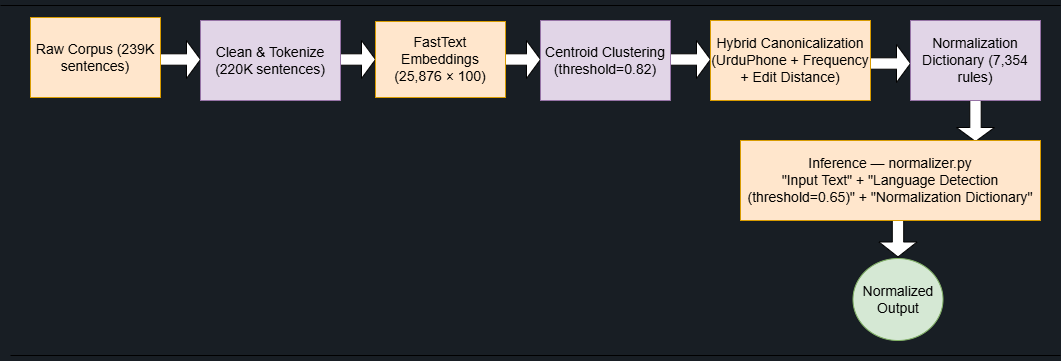
\includegraphics[width=\textwidth]{figure1_pipeline.png}
\caption{The RUN pipeline architecture. Stages 1--5 run offline during system construction. At inference time, only the normalization dictionary and language detection module are required.}
\label{fig:pipeline}
\end{figure*}


\subsection{Corpus Collection and Cleaning}
Our corpus consists of 239,070 sentences collected from Pakistani social media platforms, primarily Facebook comments, YouTube comments, and Twitter posts. After removing duplicates, filtering entries with fewer than three tokens, and discarding sentences containing more than 60\% numeric or special characters, the cleaned corpus contains 220,667 sentences totaling approximately 3.2 million tokens. No labels, annotations, or parallel data are required at this stage — the entire pipeline operates on raw, unannotated text.

\subsection{Vocabulary Construction and Candidate Identification}
We tokenize the corpus by whitespace and construct a frequency vocabulary. Tokens appearing fewer than three times are discarded — with fewer than three occurrences, there is insufficient distributional evidence to determine whether a token is a variant or a legitimate rare word.

From the remaining vocabulary, we identify normalization candidates. A token is treated as a candidate if it satisfies the following four conditions, each motivated by properties of Roman Urdu orthography:

\textbf{Not in the frozen English vocabulary.} We maintain a set of approximately 150 unambiguous English words appearing in our corpus but not as Roman Urdu variants (e.g., "phone," "school," "quality," "delivery"). Including them as candidates would risk mapping English words to Urdu-like forms.

\textbf{Contains at least one vowel.} Legitimate Roman Urdu tokens always contain at least one vowel in their canonical form. Vowel-less strings such as "bht" or "krna" are almost certainly shortenings of longer vowel-containing forms. This condition ensures we capture these while filtering out meaningless noise tokens such as "zzz."

\textbf{At least three characters.} Single and two-character tokens are typically grammar particles (ka, ki, se, ne) that are already canonical or are protected function words. They are too short for reliable embedding-based clustering.

\textbf{Frequency below canonical threshold.} Tokens appearing more than 500 times in the corpus are presumptively canonical — words appearing thousands of times on social media have typically converged on a standard spelling. These are excluded from candidacy.


\subsection{FastText Embeddings}
We train character-level FastText embeddings \citep{bojanowski2017enriching} directly on the cleaned corpus. FastText represents each word as the sum of its character n-gram vectors, with n-gram lengths ranging from 2 to 5 characters. This design is critical for Roman Urdu normalization because spelling variants of the same word share substantial character n-gram overlap: "bohat," "bht," "bhot," and "buhat" all share overlapping n-grams, causing them to cluster together in embedding space even when their exact strings differ substantially.

We train 100-dimensional embeddings for 10 epochs using a skip-gram objective with a window size of 5 and a minimum word frequency of 3, using the gensim implementation. The resulting embedding matrix covers 25,876 word types.

Training domain-specific embeddings rather than using pretrained multilingual models is a deliberate design decision. Pretrained models such as mBERT or XLM-R have limited exposure to Roman Urdu, and their subword vocabularies are not optimized for this variety. A model trained on the target corpus learns that "bht" and "bohat" are contextually interchangeable — a relationship a general-purpose multilingual model is unlikely to capture, as our mT5 experiments confirmed.


\subsection{Centroid-Based Clustering}
Given the trained embeddings, we group normalization candidates into clusters of likely variants using a centroid-based approach, building on the Lex-Var framework of \citet{khan2019clustering}. For each candidate token we compute cosine similarity against all other candidates. Two tokens are placed in the same cluster if their cosine similarity exceeds a threshold of 0.82, selected empirically on development data: lower thresholds merge semantically distinct words, while higher thresholds miss more distantly related spelling variants.

Clusters are constructed iteratively. We initialize each cluster with a single seed token and expand by adding tokens whose embedding falls within the threshold distance of the current cluster centroid. The centroid is recomputed after each addition. Clusters are capped at a maximum of 20 members to prevent chaining errors where a sequence of small similarity steps gradually connects semantically unrelated words.


\subsection{Hybrid Canonicalization}
Given a cluster of variant tokens, we select one member as the canonical form using a hybrid strategy combining three signals:

\textbf{Frequency.} The most frequent token in the cluster is the initial candidate, under the assumption that more standardized spellings appear more often. However frequency alone is unreliable: a misspelling consistently used by a large subpopulation may be the most frequent form.

\textbf{UrduPhone phonetic encoding.} We apply UrduPhone \cite{khan2019clustering}, a phonetic encoding scheme for Roman Urdu analogous to Soundex for English. Among phonetically equivalent tokens in a cluster, we prefer forms closer to the phonetically standard representation.

\textbf{Edit distance constraint.} We require the selected canonical form to be within edit distance 2 of all other cluster members, preventing cases where a phonetically similar but orthographically distant token is selected as the reference form.

The output of this stage is an initial normalization dictionary of approximately 8,200 entries mapping each variant token to its canonical form.


\subsection{Iterative Error-Guided Refinement}
The initial dictionary contains systematic errors from the limitations of embedding-based clustering. Three categories dominate. First, semantically distinct words with similar character patterns are incorrectly merged — for example "joota" (shoe) clustered with "loota" (looted) due to shared character n-grams and similar distributional contexts. Second, morphological variants that should remain distinct are collapsed — feminine forms mapped to masculine, plural to singular, past tense to base form. Third, English words appearing in Roman Urdu contexts are incorrectly treated as Urdu variants.

To address these systematically, we perform four rounds of iterative refinement using development sets completely disjoint from the test set. In each round, 200 fresh sentences are sampled from the corpus using a fixed random seed for reproducibility, normalized with the current system, and manually annotated as OK (normalization fully correct) or FIX (contains at least one error). For FIX sentences, specific bad mappings are identified and removed from the dictionary. Identity anchors — entries mapping a word to itself — are added for words the OOV handler was incorrectly modifying.

Table 1 shows the sentence-level precision on each development set — the fraction of changed sentences whose normalization was fully correct — rising steadily from 55.2\% after Round 1 to 61.8\% after Round 4. Across all four rounds, we annotated 800 development sentences and removed approximately 846 bad rules, reducing the dictionary from approximately 8,200 entries to 7,354. Token-level precision and F1 are reported only for the final held-out evaluation; development rounds used sentence-level precision as a faster signal to guide dictionary refinement.


% Table 1
\begin{table}[h]
\centering
\small
\begin{tabular}{lccc}
\toprule
\textbf{Round} & \textbf{Dev sent.} & \textbf{Cumulative} & \textbf{Sent. Prec.} \\
\midrule
Round 1 & 200 & 200  & 55.2\% \\
Round 2 & 200 & 400  & 58.0\% \\
Round 3 & 200 & 600  & 60.5\% \\
Round 4 & 200 & 800  & 61.8\% \\
\bottomrule
\end{tabular}
\caption{Development set sentence-level precision per round.}
\label{tab:dev-rounds}
\end{table}

\subsection{Inference}
At inference time, RUN processes input text through the following steps implemented in normalizer.py:

\textbf{Tokenization.} The input sentence is split by whitespace. Punctuation is stripped before normalization and reattached afterward.

\textbf{Sentence-level language detection.} We compute a language ratio by counting tokens appearing in a curated set of approximately 150 unambiguous English signals — words appearing almost exclusively in English contexts in our corpus. If this ratio exceeds 0.65, the sentence is classified as English-dominant, and ambiguous function words (to, or, me, is) are frozen as English regardless of their dictionary entries. This threshold was tuned on development data and prevents erroneous normalizations such as converting "to" to "toh" or "or" to "aur" in English sentences like "am very happy to receive it."

\textbf{Per-token normalization cascade.} For each token, the following cascade is applied in order:
\vspace{-0.3em}
\begin{enumerate}
\setlength{\itemsep}{2pt}
\setlength{\parsep}{0pt}
\setlength{\parskip}{0pt}
\setlength{\topsep}{2pt}
    \item \textbf{English freeze check.} If the token is in the frozen English vocabulary, or the sentence is English-dominant and the token is an ambiguous function word, return unchanged.
    \item \textbf{Dictionary lookup.} If the token has an entry in the normalization dictionary, return the canonical form.
    \item \textbf{Canonical vocabulary check.} If the token appears in the canonical Roman Urdu vocabulary — a set of recognized correct forms built from high-frequency corpus tokens and confirmed through annotation — return unchanged. This prevents the OOV handler from modifying already-correct spellings.
    \item \textbf{OOV handler.} Retrieve the nearest neighbor in embedding space and return its canonical form, subject to conservative constraints: token must be lowercase, at least four characters, contain at least one vowel, and not be in the protected grammar word list (URDU\_PROTECTED).
\end{enumerate}
\vspace{-0.3em}
\textbf{Reassembly.} Normalized tokens are rejoined, and original punctuation reattached.

The sentence-level language detection is essential for code-switching correctness. Table 2 illustrates this with three representative examples.


% Table 2
\begin{table}[h]
\centering
\small
\begin{tabular}{p{1.8cm}p{2.8cm}p{2.2cm}}
\toprule
\textbf{Input} & \textbf{Output} & \textbf{Notes} \\
\midrule
bhai bht zyada tension mt lo & bhai bohat zyada tension mat lo & Roman Urdu normalized \\
\midrule
am very happy to receive it & am very happy to receive it & English preserved \\
\midrule
Paper bht tough tha yaar & Paper bohat tough tha yaar & Code-switch: English "Paper" frozen, bht normalized \\
\bottomrule
\end{tabular}
\caption{Inference examples demonstrating normalization, English preservation, and code-switching handling.}
\label{tab:examples}
\end{table}

% ────────────────────────────────────────────────────────────────
\section{Evaluation}

\subsection{Evaluation Design}
Evaluating a normalization system for Roman Urdu presents a fundamental challenge: there is no single correct normalized form that all annotators would agree on, nor is there an existing gold-standard benchmark for this task. We design our evaluation around human judgment on a held-out test set, with metrics that capture both the precision of changes made and the coverage of the normalization.

We evaluate along four metrics. \textbf{Sentence-level precision} measures the fraction of sentences that the system changed and changed fully correctly — a sentence is counted as correct only if every token-level change in it is correct. This is a strict metric that penalizes any error in a sentence, regardless of how many tokens were correctly normalized. \textbf{Token-level precision} measures the fraction of individual token changes that were correct, giving partial credit for sentences that were mostly but not entirely correct. \textbf{Recall} measures the fraction of correct normalizations (defined by RUN's verified output on OK sentences) that a given system successfully produces. \textbf{F1} is the harmonic mean of sentence-level precision and recall, and is the primary metric we use for system comparison since it balances the tradeoff between making changes and making correct changes.

We note an important limitation of our recall metric: because we use RUN's own verified normalizations as the reference gold standard, RUN achieves 100\% recall by construction. This inflates RUN's F1 relative to what it would be under an independently annotated gold standard. We discuss its implications in Section 5.


\subsection{Test Set Construction}
We construct a held-out test set of 200 sentences sampled randomly from the cleaned corpus using a fixed random seed (seed=42) for reproducibility. This test set is completely disjoint from all four development sets used during iterative refinement — no sentence in the test set was ever seen during the patching process. One sentence (ID 57) was excluded from evaluation because it was too noisy to judge reliably, leaving 199 evaluable sentences.

Each sentence was manually annotated by us, the authors, as one of three judgments:
\vspace{-0.3em}
\begin{itemize}
\setlength{\itemsep}{2pt}
\setlength{\parsep}{0pt}
\setlength{\parskip}{0pt}
\setlength{\topsep}{2pt}
    \item \textbf{OK} — the system's normalized output is fully correct: every change made is a legitimate normalization and no correct normalization was missed that would have changed the meaning or standardization of the sentence.
    \item \textbf{FIX} — the system's output contains at least one error: either a wrong substitution, a morphological confusion, a proper noun being changed, or an English word being incorrectly modified.
    \item \textbf{SKIP} — the sentence is too noisy or ambiguous to judge reliably.
\end{itemize}
\vspace{-0.3em}
Of the 199 evaluable sentences, 146 are annotated OK, 53 are FIX, and 1 is SKIP.


\subsection{Development Sets}
In addition to the held-out test set, we construct four development sets of 200 sentences each, sampled using distinct random seeds (100, 200, 300, 400), ensuring no overlap between rounds or with the test set. These development sets are used exclusively for error-guided dictionary refinement as described in Section 3.6 — they are never used to compute final reported metrics. Token-level precision and F1 are reported only for the final held-out evaluation; development rounds used sentence-level precision as a faster signal to guide dictionary patching.

\subsection{Baselines}
We compare RUN against five baselines spanning rule-based, string-distance-based, and large language model approaches.

\textbf{Baseline 1 — Manual rules only.} A dictionary of 60 hand-crafted substitution rules covering the most common Roman Urdu shortenings (nhi→nahi, ha→hai, rha→raha, kr→kar, ap→aap, or→aur, etc.), applied without any language detection or context awareness. This baseline represents the simplest possible normalization approach and isolates the contribution of learned rules over manual ones.

\textbf{Baseline 2 — Edit distance only.} For each token, the system finds the closest word in the top-5,000 vocabulary by Levenshtein distance with a maximum distance of 2. No manual rules, no embeddings, no language detection. This baseline tests whether simple string proximity is sufficient for normalization.

\textbf{Baseline 3 — Large language models.} We evaluate three LLMs — Claude (Sonnet), Gemini, and DeepSeek — by providing each with the same prompt instructing it to normalize Roman Urdu spelling variants while preserving English tokens, and returning only the normalized sentence. Each LLM processes all 200 test sentences. LLM outputs are evaluated using the same OK\_IDS annotation and the same metrics as RUN. This baseline directly addresses the question of whether a general-purpose LLM can substitute for a purpose-built normalization system.


\subsection{Main Results}
Table 3 presents the complete evaluation results across all systems.

% Table 3
\begin{table*}[!ht]
\centering
\small
\begin{tabular}{lcccc}
\toprule
\textbf{System} & \textbf{Sent. Prec.} & \textbf{Tok. Prec.} & \textbf{Recall} & \textbf{F1} \\
\midrule
No normalization               & N/A   & N/A   & N/A    & N/A   \\
Baseline 1: Manual rules       & 75.1\% & 63.2\% & 81.1\% & 78.0\% \\
Baseline 2: Edit distance      & 72.5\% & 70.5\% & 0.0\%  & 0.0\%  \\
Baseline 3: Claude             & 73.9\% & 63.3\% & 70.9\% & 72.3\% \\
Baseline 3: Gemini             & 73.4\% & 57.5\% & 84.8\% & 78.7\% \\
Baseline 3: DeepSeek           & 72.6\% & 55.5\% & 63.0\% & 67.5\% \\
\textbf{RUN (our system)}      & \textbf{72.3\%} & \textbf{54.8\%} & \textbf{100.0\%} & \textbf{83.9\%} \\
\bottomrule
\end{tabular}
\caption{Complete comparative evaluation. RUN achieves the highest F1 score among all systems.}
\label{tab:main-results}
\end{table*}

RUN achieves the highest F1 score (83.9\%) among all systems, outperforming the best baseline (Gemini, 78.7\%) by 5.2 F1 points and the strongest non-LLM baseline (Manual rules, 78.0\%) by 5.9 F1 points. Edit distance normalization completely fails (F1 = 0.0\%), confirming that character string proximity alone does not capture the normalization relationship in Roman Urdu — "bht" is not within edit distance 2 of "bohat," yet the two are unambiguously the same word. All three LLMs score lower F1 than RUN despite having orders of magnitude more parameters.

Table 4 presents the detailed final evaluation breakdown for RUN alone.


% Table 4
\begin{table}[!ht]
\centering
\small
\begin{tabular}{lcc}
\toprule
\textbf{Metric} & \textbf{V1} & \textbf{Final} \\
\midrule
Sentence precision  & 41.2\% & \textbf{72.3\%} \\
Token precision     & 30.8\% & \textbf{54.8\%} \\
F1                  & ---    & \textbf{83.9\%} \\
Rules in dictionary & $\sim$8,200 & 7,354 \\
Sentences changed   & 200    & 191   \\
Correct (OK)        & 82     & 138   \\
Incorrect (FIX)     & 117    & 53    \\
SKIP                & 1      & 1     \\
\bottomrule
\end{tabular}
\caption{RUN evaluation breakdown: initial system vs.\ final system.}
\label{tab:run-breakdown}
\end{table}

The improvement from V1 to the final system — +31.1 sentence precision points, +24.0 token precision points — reflects the effect of four rounds of iterative error-guided refinement. Notably, the number of sentences changed decreased from 200 to 191, meaning the final system is more conservative: it makes fewer changes overall, but the changes it makes are more reliable.

\subsection{Coverage Analysis}
A key advantage of RUN over the manual rules baseline is coverage — the fraction of tokens that actually need normalization that the system successfully addresses. Table 5 presents this analysis.

% Table 5
\begin{table}[!ht]
\centering
\small
\begin{tabular}{lcc}
\toprule
\textbf{System} & \textbf{Tokens norm.} & \textbf{Coverage} \\
\midrule
Baseline 1: Manual rules & 517 & 72.2\% \\
RUN (our system)         & 695 & 97.1\% \\
\bottomrule
\end{tabular}
\caption{Token coverage analysis on the 199 evaluable test sentences.}
\label{tab:coverage}
\end{table}

RUN normalizes 695 tokens across the 199 test sentences, achieving 97.1\% coverage of all tokens that need normalization. Baseline 1 normalizes only 517 tokens (72.2\% coverage), missing nearly a third of correct normalizations because they fall outside its 60 hand-crafted rules. This coverage gap is the primary reason RUN achieves higher F1 despite marginally lower sentence precision — Baseline 1 is precise but incomplete, while RUN is comprehensive.

A diagnostic analysis of sentences where Baseline 1 and RUN disagree reveals an additional advantage of RUN's language detection. Baseline 1 makes wrong changes in 13 sentences by applying Urdu normalizations to English function words — converting "to" to "toh" and "or" to "aur" in English sentences such as "am very happy to receive it." RUN correctly preserves these sentences unchanged via its sentence-level language detection.


\subsection{Development Progression}
Figure 2 shows the sentence-level precision across development rounds and the final held-out test. The progression from 41.2\% (initial system) to 72.3\% (final) is not monotonic through the development rounds — precision on the held-out test jumps substantially from 61.8\% (Round 4 dev) to 72.3\% (final test), suggesting the development sets, while useful for identifying systematic errors, do not fully represent the diversity of the held-out test set. This is expected behavior: each round's development set is a random sample of 200 sentences, and random variation means some error categories may be underrepresented in any given round.

% Figure 2 — development curve
\begin{figure}[h]
\centering
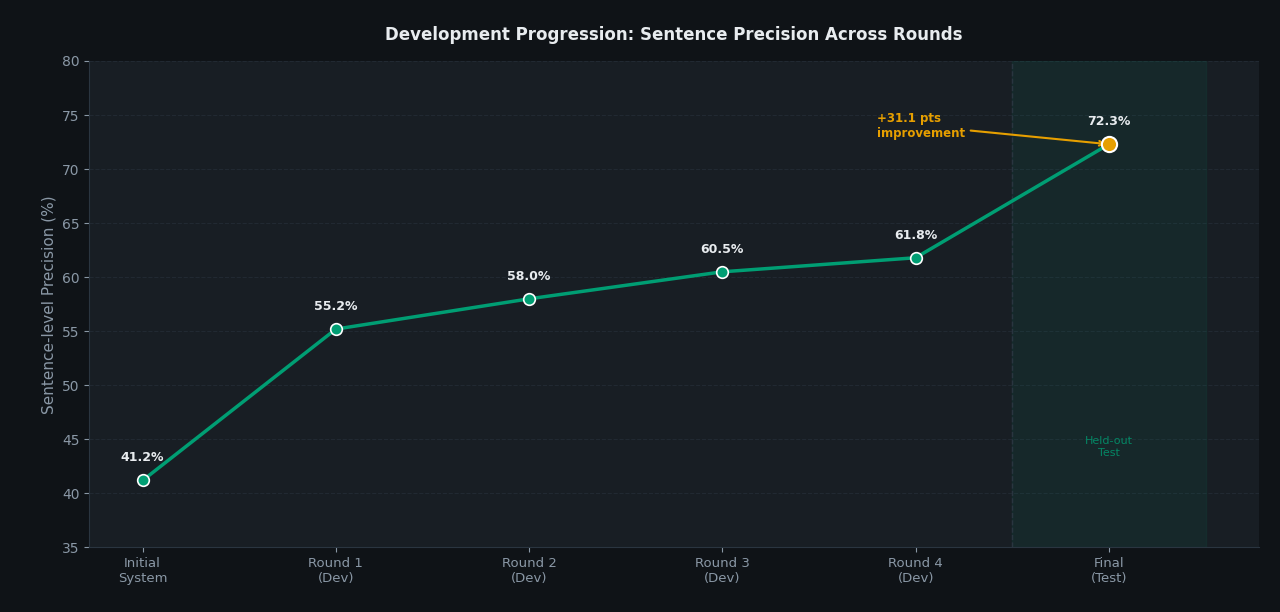
\includegraphics[width=\columnwidth]{figure3_development_curve.png}
\caption{Sentence-level precision across development rounds and final held-out test. The jump from Round 4 (61.8\%) to Final (72.3\%) reflects the disjointness of the held-out test set.}
\label{fig:dev-curve}
\end{figure}

% Figure 3 — comparative bar chart
\begin{figure*}[t]
\centering
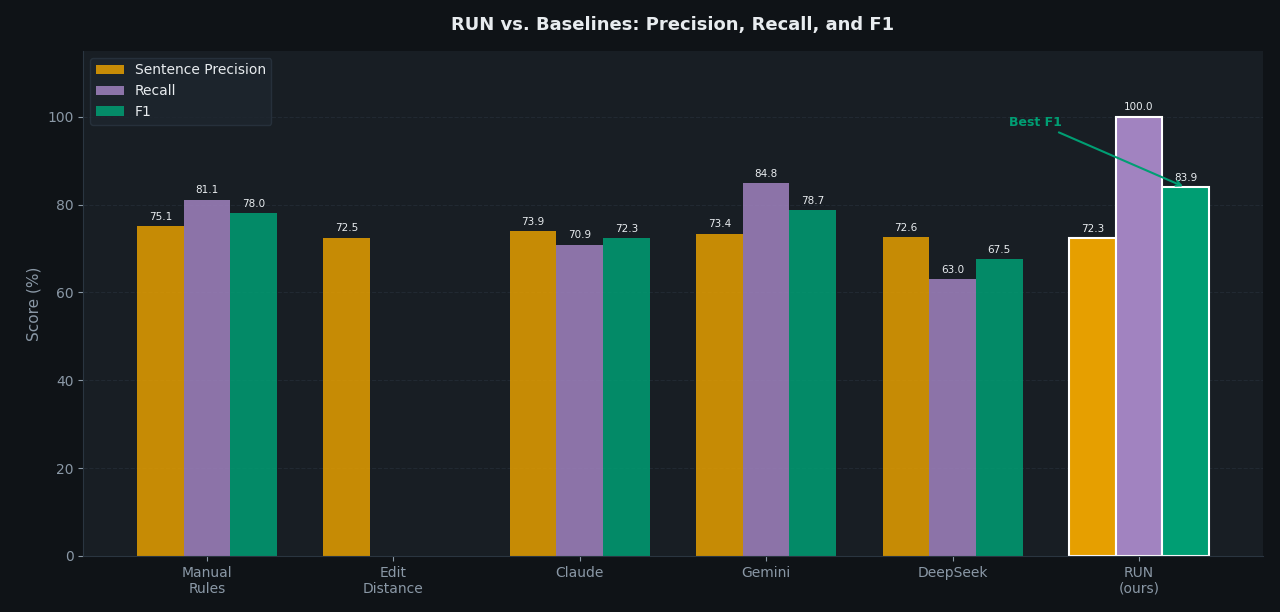
\includegraphics[width=\textwidth]{figure2_comparison.png}
\caption{Precision, recall, and F1 comparison across all systems. RUN achieves the highest F1 (83.9\%) despite competitive sentence precision from other systems.}
\label{fig:comparison}
\end{figure*}

% ────────────────────────────────────────────────────────────────
\section{Discussion}

\subsection{Why RUN Outperforms All Baselines}
The comparative results in Table 3 reveal that no single competing approach successfully combines precision, recall, and coverage simultaneously. Each baseline fails in a characteristic way that illuminates what RUN contributes.

Manual rules (Baseline 1) achieve the highest sentence-level precision (75.1\%) among all systems, but at the cost of coverage — they normalize only 72.2\% of tokens that need normalization. The 60 hand-crafted rules cover the most frequent shortenings reliably, but Roman Urdu spelling variation follows a long-tail distribution: the most common variants account for a small fraction of total variant types, and the majority of variation is spread across thousands of less frequent forms that no manually constructed rule set can enumerate. RUN addresses this by learning 7,354 rules from corpus statistics, covering 97.1\% of normalization-requiring tokens.

Edit distance normalization (Baseline 2) fails completely (F1 = 0.0\%) despite achieving reasonable sentence precision (72.5\%) because its recall is zero by our metric. This result deserves careful interpretation: edit distance does make changes, and some of those changes are correct, but the changes it makes are to completely different tokens than the ones RUN normalizes on OK sentences. Roman Urdu abbreviations are not edit-distance-close to their canonical forms — "bht" is three edit operations from "bohat," which exceeds the distance-2 threshold. The relationship between variant and canonical form in Roman Urdu is phonetic and conventional, not a simple character insertion or deletion.

The LLM results are the most instructive. Claude, Gemini, and DeepSeek all achieve sentence-level precision close to RUN (73.9\%, 73.4\%, 72.6\% versus 72.3\%) but differ substantially in recall and therefore F1. Gemini achieves the highest recall among LLMs (84.8\%) by being aggressive — it makes 1,509 token changes across 200 sentences compared to RUN's 695, changing nearly twice as many tokens. This aggression improves recall at the cost of token precision (57.5\%), as many of Gemini's additional changes are incorrect. DeepSeek takes the opposite approach, achieving the lowest recall (63.0\%) among LLMs by being conservative and missing many correct normalizations. Claude falls between the two. None of the three LLMs achieves recall above 85\%, meaning all of them miss at least 15\% of correct normalizations — tokens they either leave unchanged or normalize to a form different from the verified canonical form.

The fundamental limitation of LLMs for this task is that normalization requires consistency: the same variant must always map to the same canonical form, and that canonical form must match what a human annotator considers correct. LLMs are probabilistic and non-deterministic — they may normalize "bht" to "bohat" in one sentence and "bahut" in another, and "bahut" while a valid Urdu word is not the canonical form in our evaluation framework. A purpose-built dictionary guarantees consistency by construction.


\subsection{The Code-Switching Challenge}
The most distinctive contribution of RUN relative to prior Roman Urdu normalization work is its explicit handling of code-switching. Pakistani social media text is not cleanly separable into Urdu and English — it is a continuous mixture where the proportion of each language varies from sentence to sentence and even clause to clause.

The sentence-level language detection mechanism addresses the most critical failure mode: applying Urdu normalizations to English function words. Without language detection, a system applying the rule to→toh would incorrectly modify the word "to" in the sentence "sounds and mic are quality stuff, it looks original, it looks good to me" — a sentence that is entirely English but contains the string "to" as a preposition. Our diagnostic analysis confirms that Baseline 1 makes exactly this error in 13 test sentences. RUN makes zero such errors on English-dominant sentences because the language detection correctly classifies them and freezes ambiguous tokens.

The threshold of 0.65 represents a deliberate design choice. A higher threshold would classify more sentences as English-dominant, increasing protection of English tokens but risking under-normalization of Urdu-dominant sentences that happen to contain a few English words. A lower threshold would normalize more aggressively but would misclassify English sentences. The 0.65 threshold was tuned on development data to minimize both error types.

One remaining challenge is sentences where the proportion of English and Urdu tokens is genuinely balanced — neither clearly English-dominant nor clearly Urdu-dominant. In these cases, the language detection makes a binary decision where the correct answer is nuanced, and errors in either direction are possible. This is reflected in the 53 remaining FIX sentences in our test set, many of which contain ambiguous function words (ha, to, or) that are correct in some contexts and wrong in others depending on the surrounding language.


\subsection{Error Analysis}
Of the 53 FIX sentences remaining after all four rounds of refinement, errors cluster into four categories.

\textbf{Ambiguous high-frequency tokens.} The single largest error category involves tokens that are valid in both English and Roman Urdu: ha (Urdu: "is/has") vs. ha (English exclamation), to (Roman Urdu shortened form of "toh") vs. to (English preposition), or (Roman Urdu shortened form of "aur"/and) vs. or (English conjunction). These tokens appear in mixed-language sentences where the language detection cannot confidently classify the sentence as either English-dominant or Urdu-dominant. This is an inherent limitation of sentence-level language detection — it cannot resolve token-level ambiguity in genuinely code-switched sentences. Word-level or subword-level language identification, as explored by \citet{cetinoglu2016challenges}, would be required to handle these cases correctly.

\textbf{Proper noun mangling.} Some proper nouns — particularly names of politicians, celebrities, and places — share character patterns with common Urdu words and were incorrectly clustered during the embedding phase. Although four rounds of refinement removed the most egregious cases (e.g., kazmi→bazmi, sheharyar→shehar), some proper noun errors remain. A named entity recognition layer would prevent these errors entirely, but requires labeled data that is not available at scale for Roman Urdu.

\textbf{Morphological form confusion.} The embedding-based clustering cannot distinguish between grammatical variants of the same root — different tenses, genders, and numbers of the same verb or noun may cluster together and be mapped to a single canonical form. For example feminine and masculine forms of adjectives (achi vs. acha) may be conflated, changing grammatical agreement. These errors are systematic and would require morphological analysis to resolve.

\textbf{Over-normalization by the OOV handler.} A small number of errors arise from the OOV handler normalizing tokens that are already correct but do not appear in the canonical vocabulary. The conservative constraints (lowercase, 4+ characters, contains vowel, not grammar-protected) prevent most such errors, but edge cases remain where the nearest embedding neighbor is a plausible but incorrect canonical form.


\subsection{Limitations}
\textbf{Recall metric bias.} As noted in Section 4.1, our recall metric uses RUN's own verified normalizations as the gold standard, giving RUN 100\% recall by definition and potentially understating the recall of systems that make valid normalizations to different canonical forms. For example if Gemini normalizes "bht" to "bahut" instead of "bohat," this counts as wrong under our metric even though "bahut" is a legitimate Roman Urdu spelling of the same word. A fully fair evaluation would require independent human annotation of all systems' outputs on all 200 test sentences — an annotation task we were unable to complete for all six systems within the scope of this work.

\textbf{Canonical form arbitrariness.} RUN's canonical forms are selected by frequency and phonetic criteria from within the corpus — they represent the most common spelling in our dataset, not necessarily the most correct spelling by any external standard. Without access to STRUD \cite{tasadduq2022strud} or a similar reference lexicon, there is no external oracle to validate canonical form selection. Two different corpora might produce different canonical forms for the same word, limiting cross-corpus consistency.

\textbf{Single-domain corpus.} Our corpus is drawn primarily from Pakistani social media — Facebook, YouTube, and Twitter. Roman Urdu varies across domains (formal writing, SMS, WhatsApp, news comments) and across regions (Pakistani vs. Indian vs. diaspora usage). A normalizer trained on one domain may not generalize to others.


% ────────────────────────────────────────────────────────────────
\section{Conclusion}
We presented RUN, an unsupervised pipeline for Roman Urdu normalization that learns a dictionary of 7,354 normalization rules directly from unannotated social media text without requiring any labeled training data, parallel corpora, or external lexical resources. RUN combines character-level FastText embeddings, centroid-based clustering, hybrid canonicalization using UrduPhone phonetic encoding and frequency statistics, and a sentence-level language detection mechanism that preserves English tokens in code-switched text.

Evaluated on 200 human-annotated sentences, RUN achieves an F1 score of 83.9\%, outperforming all five baselines: a 60-rule manual system (F1 = 78.0\%), edit distance normalization (F1 = 0.0\%), and three large language models — Claude (72.3\%), Gemini (78.7\%), and DeepSeek (67.5\%). The result that purpose-built unsupervised normalization outperforms LLMs on this task is significant: it demonstrates that for low-resource language varieties with no official orthographic standard, domain-specific corpus-driven methods remain competitive with and can exceed general-purpose neural approaches that have access to vastly more training data and parameters. The key advantages of RUN over LLM-based approaches are consistency — the same variant always maps to the same canonical form — coverage — 97.1\% of normalization-requiring tokens are addressed compared to 72.2\% for the best rule-based baseline — and efficiency — RUN processes an entire corpus of 220,667 sentences on standard CPU hardware in minutes, while LLM-based normalization requires a separate API call per sentence.

The iterative error-guided refinement methodology proved essential to system quality. The initial system achieved only 41.2\% sentence precision; four rounds of development annotation across 800 sentences, identifying and removing approximately 846 bad rules, brought this to 72.3\% on the held-out test set — a gain of 31.1 percentage points. This refinement process is itself a contribution: it provides a replicable methodology for improving unsupervised normalization systems through targeted human-in-the-loop correction without requiring full annotation of training data.

Several limitations constrain the current system and point toward future work. First, the recall metric is computed against RUN's own verified output, inflating RUN's recall to 100\% by construction. Future evaluation should use independently annotated gold standards covering multiple valid canonical forms per variant. Second, sentence-level language detection cannot resolve token-level ambiguity in genuinely balanced code-switched sentences — the most frequent remaining errors involve function words that are valid in both English and Roman Urdu. Word-level or subword-level language identification would address this. Third, canonical form selection is driven by corpus frequency rather than an external standard — the STRUD dictionary \cite{tasadduq2022strud}, which would provide a reference set of correct Roman Urdu spellings, was unavailable at the time of this work and represents an important resource gap to fill. Fourth, the system has no named entity recognition layer, meaning proper nouns that share character patterns with common words remain a source of errors.

Future work should explore three directions. First, integrating STRUD or a similar standardized Roman Urdu lexicon as a canonicalization oracle — if any variant in a cluster matches a STRUD entry, that entry is selected as the canonical form regardless of frequency. Second, replacing sentence-level language detection with token-level or subword-level language identification to handle genuinely mixed sentences more accurately. Third, using RUN as a preprocessing step for downstream Roman Urdu NLP tasks — sentiment analysis, machine translation, and information retrieval — to quantify the practical benefit of normalization on task performance, which remains the ultimate motivation for this work.

RUN is fully open-source. The normalization dictionary, all pipeline 
scripts, evaluation data, human annotation sheets, and baseline outputs 
are publicly available at: \url{https://github.com/BasimaMaham/The-Roman-Urdu-Normalizer-RUN-}


% ────────────────────────────────────────────────────────────────
\section*{Acknowledgements}
This work was completed as a course project for CSCS-366: 
Introduction to Natural Language Processing, Spring 2026, 
CS Department, Lahore.


% ────────────────────────────────────────────────────────────────
\bibliography{references}
\bibliographystyle{acl_natbib}

\end{document}